\documentclass{article}
\usepackage{graphicx}
\usepackage{amsmath,amsthm,amssymb}
\usepackage[font=small,labelfont=bf]{caption}
\usepackage{tikz}
\usepackage{pgfplots}
\pgfplotsset{compat=1.18}
\usetikzlibrary{calc, angles, quotes, shapes.geometric, decorations.pathreplacing}
\usepackage{tkz-euclide}
\usepackage[inline]{asymptote}
\usepackage{float}
\usepackage[margin=1in]{geometry}
\usepackage{gensymb}
\usepackage[normalem]{ulem}
\usepackage{hyperref}
\hypersetup{
    colorlinks=true,
    linkcolor=blue,
    filecolor=magenta,      
    urlcolor=cyan,
    pdftitle={Overleaf Example},
    pdfpagemode=FullScreen,
    }
\usepackage{fancyhdr}
\pagestyle{fancy}
\fancyhead[R]{Enoch Yu}
\pagenumbering{gobble}
\usepackage{enumitem}
\newtheorem{theorem}{Theorem}[section]
\newtheorem{lemma}[theorem]{Lemma}
\newtheorem*{lemma*}{Lemma}
\newtheorem{sublemma}{Lemma}[section]
\newtheorem{proposition}{Proposition}
\newtheorem{corollary}{Corollary}[theorem]
\newtheorem{example}{Example}[section]
\newtheorem*{example*}{Example}
\newenvironment{solution}{\begin{trivlist}\item[]{\bf Solution}}{\qed \end{trivlist}}
\newcommand{\verteq}{\rotatebox{90}{$\;\;=\;\;$}}
\newcommand*\circled[1]{\tikz[baseline=(char.base)]{
            \node[shape=circle,draw,inner sep=1pt] (char) {#1};}}
\newcommand{\triangled}[1]{\tikz[baseline=(char.base)]{
            \node[shape=regular polygon, regular polygon sides=3, draw, inner sep=0.2pt] (char) {#1};}}

\title{Problem Set 30}
\author{Enoch Yu}
\date{July 2025}

\begin{document}

\section*{2005 AIME II Problem 12}
Square $ABCD$ has center $O$ and $AB = 900$. Points $E$ and $F$ are on $\overline{AB}$ with $AE < BF$ and $E$ between $A$ and $F$ such that $\angle{EOF} = 45^\circ$ and $EF = 400$. Find $BF$.
\begin{solution}
\\\\
\begin{minipage}{0.5\textwidth}
\begin{center}
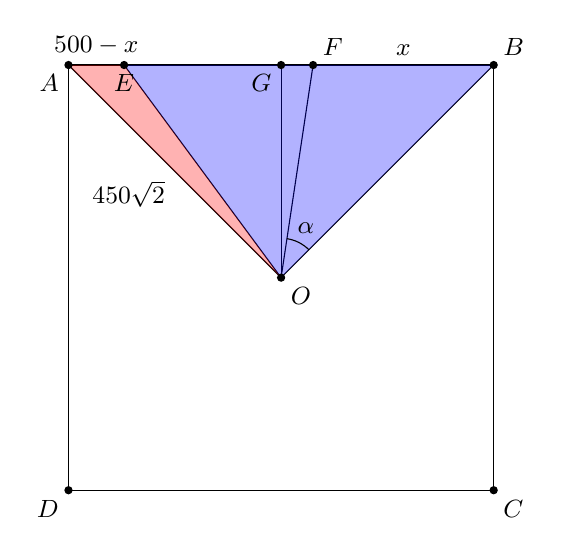
\begin{tikzpicture}[scale=0.6, every node/.style={font=\small}]
    \coordinate (A) at (0,9);
    \coordinate (B) at (9,9);
    \coordinate (C) at (9,0);
    \coordinate (D) at (0,0);
    \coordinate (E) at ({2.5-0.5*sqrt(7)},9);
    \coordinate (F) at ({6.5-0.5*sqrt(7)},9);
    \coordinate (G) at (4.5,9);
    \coordinate (O) at (4.5,4.5);
    
    \draw (A) -- (B) -- (C) -- (D) -- cycle;
    
    \draw (E) -- (O) -- (F);
    \draw (G) -- (O);
    \draw (A) -- (O) -- (B);

    \fill[red, opacity=0.3] (A) -- (O) -- (E);
    \fill[blue, opacity=0.3] (O) -- (E) -- (B);
    
    \foreach \p in {A,B,C,D,E,F,G,O}
    \fill (\p) circle (2.5pt);
    
    \node[below left] at (A) {$A$};
    \node[above right] at (B) {$B$};
    \node[below right] at (C) {$C$};
    \node[below left] at (D) {$D$};
    \node[below] at (E) {$E$};
    \node[above right] at (F) {$F$};
    \node[below left] at (G) {$G$};
    \node[below right] at (O) {$O$};

    \draw pic["$\alpha$", draw=black, angle radius=0.5cm, angle eccentricity=1.4] {angle=B--O--F};
    
    \node[above] at ($0.5*(F)+0.5*(B)$) {$x$};
    \node[above] at ($0.5*(A)+0.5*(E)$) {$500 - x$};
    \node[below left] at ($(A)!0.5!(O)$) {$450\sqrt{2}$};
\end{tikzpicture}
\end{center}
\end{minipage}
\begin{minipage}{0.5\textwidth}
The Law of Sines could be utilized.
\begin{align*}
    \frac{EO}{\sin45^\circ} &= \frac{450\sqrt{2}}{\sin\angle{AEO}} = \frac{500 - x}{\sin(45 - \alpha)} \\
    \frac{EO}{\sin45^\circ} &= \frac{450\sqrt{2}}{\sin\angle{OEB}} = \frac{400 + x}{\sin(45 + \alpha)} = \frac{400 + x}{\cos(45 - \alpha)}
\end{align*}
\begin{align*}
    \frac{500 - x}{\sin(45 - \alpha)} &= \frac{400 + x}{\cos(45 - \alpha)} \\
    \frac{500 - x}{400 + x} &= \tan(45 - \alpha)
\end{align*}
\end{minipage}
\begin{minipage}{0.5\textwidth}
\begin{center}
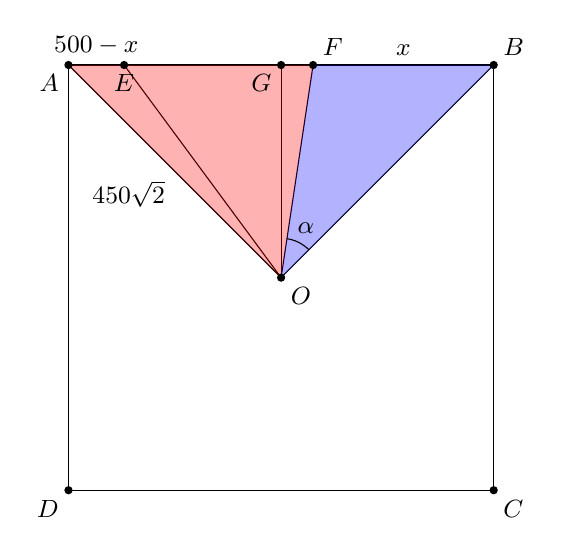
\begin{tikzpicture}[scale=0.6, every node/.style={font=\small}]
    \coordinate (A) at (0,9);
    \coordinate (B) at (9,9);
    \coordinate (C) at (9,0);
    \coordinate (D) at (0,0);
    \coordinate (E) at ({2.5-0.5*sqrt(7)},9);
    \coordinate (F) at ({6.5-0.5*sqrt(7)},9);
    \coordinate (G) at (4.5,9);
    \coordinate (O) at (4.5,4.5);
    
    \draw (A) -- (B) -- (C) -- (D) -- cycle;
    
    \draw (E) -- (O) -- (F);
    \draw (G) -- (O);
    \draw (A) -- (O) -- (B);

    \fill[red, opacity=0.3] (A) -- (O) -- (F);
    \fill[blue, opacity=0.3] (O) -- (F) -- (B);
    
    \foreach \p in {A,B,C,D,E,F,G,O}
    \fill (\p) circle (2.5pt);
    
    \node[below left] at (A) {$A$};
    \node[above right] at (B) {$B$};
    \node[below right] at (C) {$C$};
    \node[below left] at (D) {$D$};
    \node[below] at (E) {$E$};
    \node[above right] at (F) {$F$};
    \node[below left] at (G) {$G$};
    \node[below right] at (O) {$O$};
    
    \draw pic["$\alpha$", draw=black, angle radius=0.5cm, angle eccentricity=1.4] {angle=B--O--F};
    
    \node[above] at ($0.5*(F)+0.5*(B)$) {$x$};
    \node[above] at ($0.5*(A)+0.5*(E)$) {$500 - x$};
    \node[below left] at ($(A)!0.5!(O)$) {$450\sqrt{2}$};
\end{tikzpicture}
\end{center}
\end{minipage}
\begin{minipage}{0.5\textwidth}
The Law of Sines could be utilized.
\begin{align*}
    \frac{900 - x}{\sin(90 - \alpha)} &= \frac{x}{\sin(\alpha)} \\
    \frac{x}{900 - x} &= \tan\alpha
\end{align*}
\end{minipage}
\\\\\\
The addition property of $\tan$ could be used to compute for $x$.
\begin{align*}
    \frac{500 - x}{400 + x} &= \frac{1 - \frac{x}{900 - x}}{1 + \frac{x}{900 - x}} \\
    \frac{500 - x}{400 + x} &= \frac{900 - x - x}{900 - x + x} \\
    900(500 - x) &= (900 - 2x)(400 + x) \\
    450000 - 900x &= 360000 + 100x - 2x^2 \\
    x^2 - 500x + 45000 &= 0 \\
    \therefore x &= \boxed{250 + 50\sqrt{7}}
\end{align*}
\end{solution}

\newpage
\section*{2009 AIME II Problem 5}
Equilateral triangle $T$ is inscribed in circle $A$, which has radius $10$. Circle $B$ with radius $3$ is internally tangent to circle $A$ at one vertex of $T$. Circles $C$ and $D$, both with radius $2$, are internally tangent to circle $A$ at the other two vertices of $T$. Circles $B$, $C$, and $D$ are all externally tangent to circle $E$. Find the radius of circle $E$.
\begin{center}
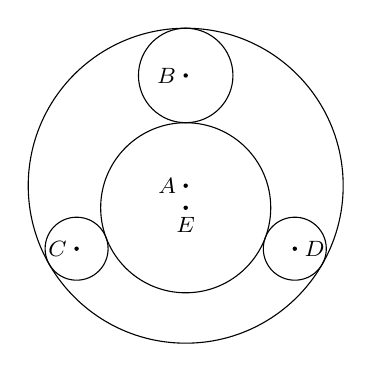
\begin{tikzpicture}[scale=0.2]
    \coordinate (A) at (0,0);
    \coordinate (B) at (0,7);
    \coordinate (C) at ({-8*cos(30)},{-8*sin(30)});
    \coordinate (D) at ({8*cos(30)},{-8*sin(30)});
    \coordinate (E) at (0,{4-27/5});
    
    \draw (A) circle (10);
    \draw (B) circle (3);
    \draw (C) circle (2);
    \draw (D) circle (2);
    \draw (E) circle ({27/5});
    
    \fill (A) circle (4pt);
    \fill (B) circle (4pt);
    \fill (C) circle (4pt);
    \fill (D) circle (4pt);
    \fill (E) circle (4pt);
    
    \node[left] at (A) {\footnotesize $A$};
    \node[left] at (B) {\footnotesize $B$};
    \node[left] at (C) {\footnotesize $C$};
    \node[right] at (D) {\footnotesize $D$};
    \node[below] at (E) {\footnotesize $E$};
\end{tikzpicture}
\end{center}
\begin{solution}
Consider $\triangle{AED}$, and let the radius of circle $E$ be $r$. Using the law of cosines for $\angle{DAE}$, the following equations could be written.
\begin{align*}
    \cos60^\circ &= \frac{(r - 4)^2 + 8^2 - (r + 2)^2}{2 \cdot (r - 4) \cdot 8} \\
    8r - 32 &= -12r + 76 \\
    \therefore r&= \boxed{\frac{27}{5}}
\end{align*}
\end{solution}

\section*{Problem}
The perimeter of a triangle is numerically $12$ times the average of the sines of the angles of the triangle. If one side of the triangle has length $2$, what are the possible measures of the angle opposite that side?
\begin{solution}
Let $a, b, c$ be the side lengths of the opposite sides of the angle $A, B, C$. WLOG, let $c = 2$. The following equations could be written.
\begin{align*}
    a + b + c &= 4(\sin A + \sin B + \sin C) \\
    2 + a + b &= 4 \left( \frac{a}{2} \sin C + \frac{b}{2} \sin C + \sin C \right) \quad \left( \because \frac{\sin A}{a} = \frac{\sin B}{b} = \frac{\sin C}{2} \right) \\
    \sin C &= \frac{1}{2} \\
    \therefore C &= \boxed{30^\circ, 150^\circ}
\end{align*}
\end{solution}

\newpage
\section*{1983 AHSME Problem 30}
Distinct points $A$ and $B$ are on a semicircle with diameter $\overline{MN}$ and center $C$. The point $P$ is on $\overline{CN}$ and $\angle{CAP} = \angle{CBP} = 10^\circ$. If $\stackrel{\frown}{MA} = 40^\circ$, then what is $\stackrel{\frown}{BN}$?
\begin{solution}
\begin{center}
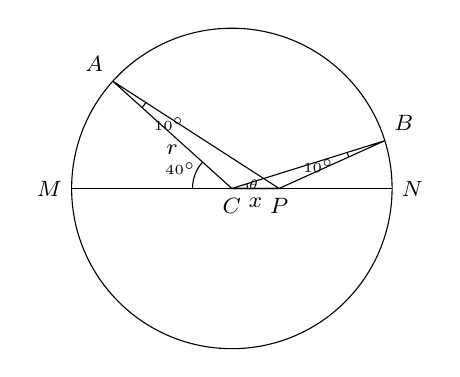
\begin{tikzpicture}[scale=0.3]
    \coordinate (A) at (-5.04, 4.54);
    \coordinate (B) at (6.47, 2.02);
    \coordinate (C) at (0, 0);
    \coordinate (P) at (2, 0);
    \coordinate (M) at (-6.78306715284, 0);
    \coordinate (N) at (6.78306715284, 0);

    \draw (A) -- (C) -- (P) -- cycle;
    \draw (C) -- (P) -- (B) -- cycle;
    \draw (C) circle (6.78306715284);
    \draw (M) -- (N);

    \draw pic["\tiny $\theta$", draw=black, angle radius=0.2cm, angle eccentricity=1.4] {angle=P--C--B};
    \draw pic["\tiny $10^\circ$", draw=black, angle radius=0.5cm, angle eccentricity=1.8] {angle=C--A--P};
    \draw pic["\tiny $10^\circ$", draw=black, angle radius=0.5cm, angle eccentricity=1.8] {angle=C--B--P};
    \draw pic["\tiny $40^\circ$", draw=black, angle radius=0.5cm, angle eccentricity=1.4] {angle=A--C--M};

    \node[below] at ($(C)!0.5!(P)$) {\footnotesize $x$};
    \node[above left] at (A) {\footnotesize $A$};
    \node[above right] at (B) {\footnotesize $B$};
    \node[below] at (C) {\footnotesize $C$};
    \node[below] at (P) {\footnotesize $P$};
    \node[left] at (M) {\footnotesize $M$};
    \node[right] at (N) {\footnotesize $N$};
    \node[below] at ($(A)!0.5!(C)$) {\footnotesize $r$};
\end{tikzpicture}
\end{center}
Using the law of sines, the following equation is evident.
\[
\frac{\sin\angle{APC}}{r} = \frac{\sin10^\circ}{x} = \frac{\sin\angle{CPB}}{r}
\]
Because $A$ and $B$ are distinct points and $\sin\angle{APC} = \sin\angle{CPB}$ with $\angle{APC} = 30^\circ$, $\angle{CPB}$ must be $150^\circ$. In other words, $\theta = \boxed{20^\circ}$.
\end{solution}

\end{document}
